\documentclass[tikz,border=5pt]{standalone}
\usepackage[english]{babel}
\usepackage[utf8]{inputenc}
\usepackage[T1]{fontenc}
\usepackage{lmodern}
\usetikzlibrary{arrows.meta}

\begin{document}
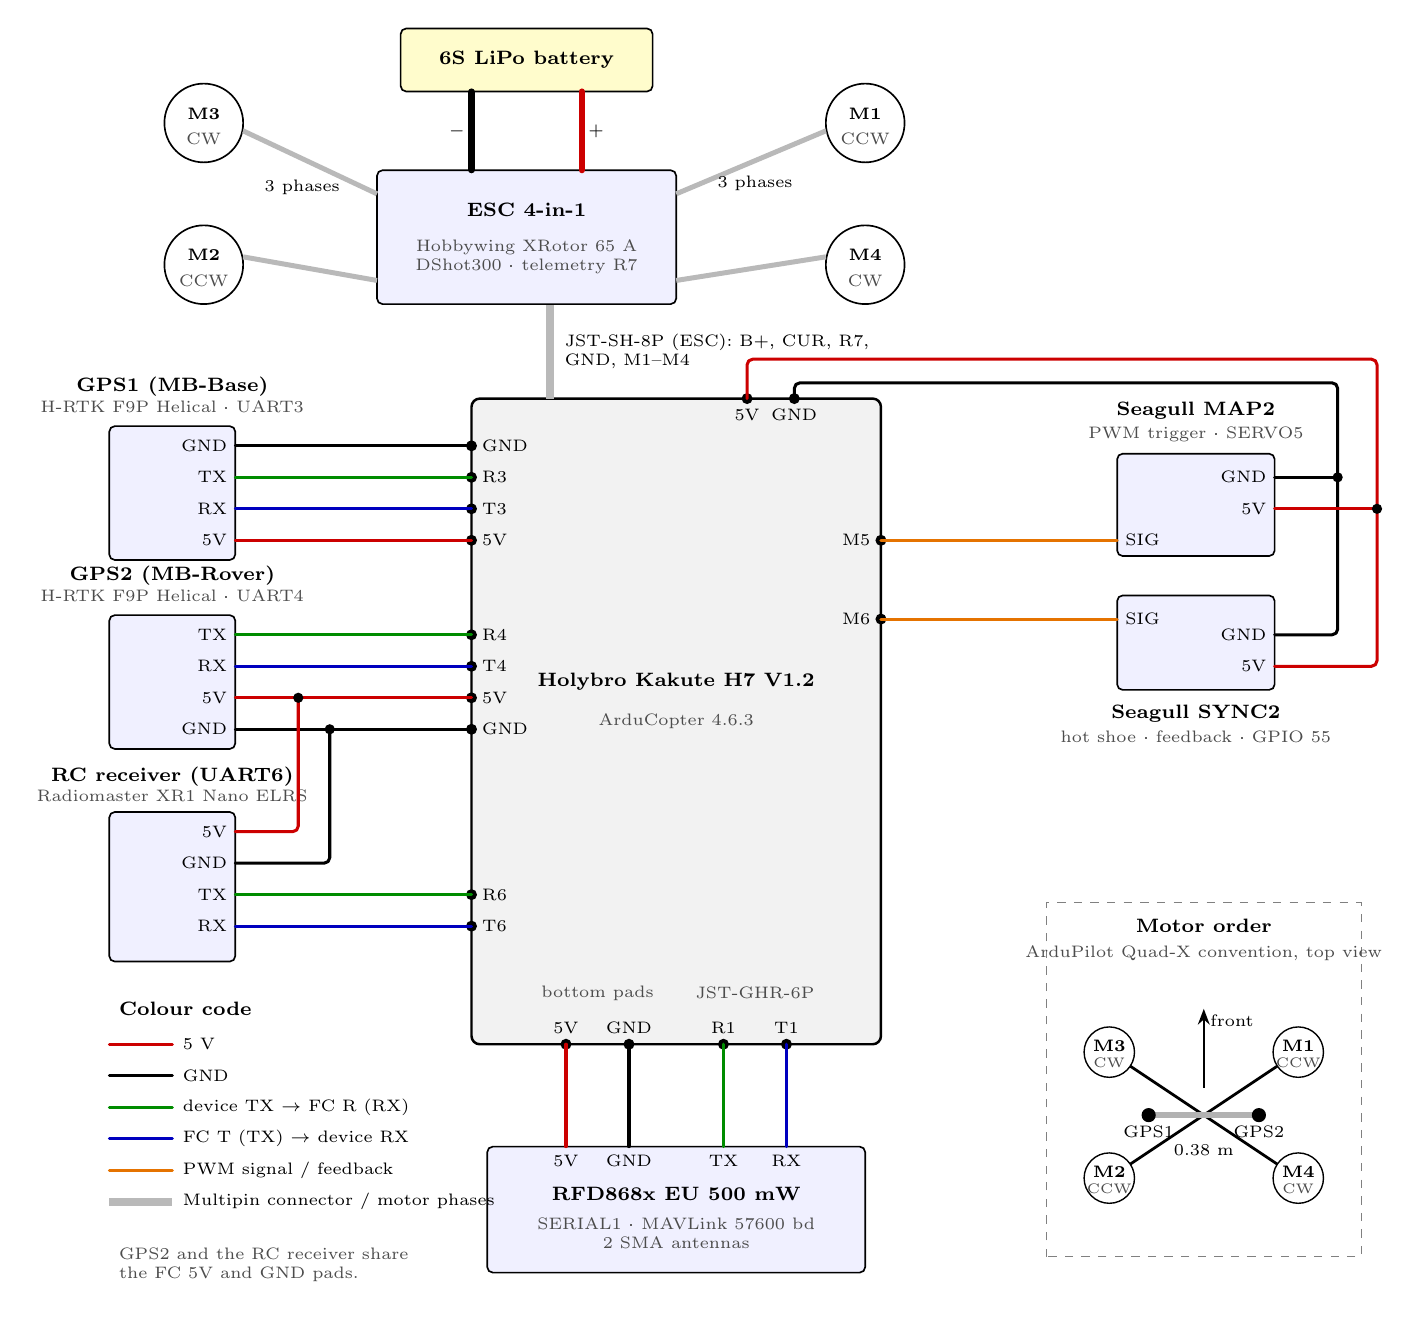
\begin{tikzpicture}[x=1cm,y=1cm,font=\fontsize{7}{8}\selectfont,
    dev/.style={draw,rounded corners=2pt,fill=blue!6,line width=0.6pt},
    fcs/.style={draw,rounded corners=3pt,fill=gray!10,line width=0.9pt},
    w/.style={line width=1.1pt,line cap=round,line join=round,rounded corners=2pt},
    r5/.style={w,red!80!black}, g0/.style={w,black},
    rxl/.style={w,green!55!black}, txl/.style={w,blue!75!black}, sg/.style={w,orange!90!black},
    ph/.style={line width=3pt,gray!55,line cap=butt},
    pin/.style={font=\fontsize{6}{7}\selectfont,inner sep=0.8pt},
    ttl/.style={font=\bfseries\fontsize{7}{8}\selectfont,align=center},
    sub/.style={font=\fontsize{6}{7}\selectfont,align=center,text=black!70}]

% ---------------- macros ----------------
\newcommand{\padL}[3]{\fill[black] (#1,#2) circle (0.07); \node[pin,anchor=west] at (#1+0.1,#2) {#3};}
\newcommand{\padR}[3]{\fill[black] (#1,#2) circle (0.07); \node[pin,anchor=east] at (#1-0.1,#2) {#3};}
\newcommand{\padT}[3]{\fill[black] (#1,#2) circle (0.07); \node[pin,anchor=north] at (#1,#2-0.1) {#3};}
\newcommand{\padB}[3]{\fill[black] (#1,#2) circle (0.07); \node[pin,anchor=south] at (#1,#2+0.1) {#3};}
\newcommand{\jn}[2]{\fill (#1,#2) circle (0.065);}
\newcommand{\pinE}[3]{\node[pin,anchor=east] at (#1-0.07,#2) {#3};}
\newcommand{\pinW}[3]{\node[pin,anchor=west] at (#1+0.07,#2) {#3};}
\newcommand{\pinN}[3]{\node[pin,anchor=north] at (#1,#2-0.07) {#3};}

% ---------------- controlador de vol ----------------
\draw[fcs] (-2.6,-4.2) rectangle (2.6,4.0);
\node[ttl] at (0,0.4) {Holybro Kakute H7 V1.2};
\node[sub] at (0,-0.1) {ArduCopter 4.6.3};

\padL{-2.6}{3.4}{GND}  \padL{-2.6}{3.0}{R3}  \padL{-2.6}{2.6}{T3}  \padL{-2.6}{2.2}{5V}
\padL{-2.6}{1.0}{R4}   \padL{-2.6}{0.6}{T4}  \padL{-2.6}{0.2}{5V}  \padL{-2.6}{-0.2}{GND}
\padL{-2.6}{-2.3}{R6}  \padL{-2.6}{-2.7}{T6}
\padR{2.6}{2.2}{M5}    \padR{2.6}{1.2}{M6}
\padT{0.9}{4.0}{5V}    \padT{1.5}{4.0}{GND}
\padB{-1.4}{-4.2}{5V}  \padB{-0.6}{-4.2}{GND}  \padB{0.6}{-4.2}{R1}  \padB{1.4}{-4.2}{T1}
\node[sub] at (-1.0,-3.55) {bottom pads};
\node[sub] at (1.0,-3.55) {JST-GHR-6P};

% ---------------- GPS1 ----------------
\draw[dev] (-7.2,1.95) rectangle (-5.6,3.65);
\node[ttl] at (-6.4,4.15) {GPS1 (MB-Base)};
\node[sub] at (-6.4,3.9) {H-RTK F9P Helical · UART3};
\pinE{-5.6}{3.4}{GND}\pinE{-5.6}{3.0}{TX}\pinE{-5.6}{2.6}{RX}\pinE{-5.6}{2.2}{5V}
\draw[g0]  (-5.6,3.4) -- (-2.6,3.4);
\draw[rxl] (-5.6,3.0) -- (-2.6,3.0);
\draw[txl] (-5.6,2.6) -- (-2.6,2.6);
\draw[r5]  (-5.6,2.2) -- (-2.6,2.2);

% ---------------- GPS2 ----------------
\draw[dev] (-7.2,-0.45) rectangle (-5.6,1.25);
\node[ttl] at (-6.4,1.75) {GPS2 (MB-Rover)};
\node[sub] at (-6.4,1.5) {H-RTK F9P Helical · UART4};
\pinE{-5.6}{1.0}{TX}\pinE{-5.6}{0.6}{RX}\pinE{-5.6}{0.2}{5V}\pinE{-5.6}{-0.2}{GND}
\draw[rxl] (-5.6,1.0) -- (-2.6,1.0);
\draw[txl] (-5.6,0.6) -- (-2.6,0.6);
\draw[r5]  (-5.6,0.2) -- (-2.6,0.2);
\draw[g0]  (-5.6,-0.2) -- (-2.6,-0.2);

% ---------------- receptor ELRS ----------------
\draw[dev] (-7.2,-3.15) rectangle (-5.6,-1.25);
\node[ttl] at (-6.4,-0.8) {RC receiver (UART6)};
\node[sub] at (-6.4,-1.05) {Radiomaster XR1 Nano ELRS};
\pinE{-5.6}{-1.5}{5V}\pinE{-5.6}{-1.9}{GND}\pinE{-5.6}{-2.3}{TX}\pinE{-5.6}{-2.7}{RX}
\draw[r5] (-5.6,-1.5) -- (-4.8,-1.5) -- (-4.8,0.2);
\draw[g0] (-5.6,-1.9) -- (-4.4,-1.9) -- (-4.4,-0.2);
\draw[rxl] (-5.6,-2.3) -- (-2.6,-2.3);
\draw[txl] (-5.6,-2.7) -- (-2.6,-2.7);
\jn{-4.8}{0.2}\jn{-4.4}{-0.2}

% ---------------- ESC, bateria i motors ----------------
\draw[ph] (-1.6,4.0) -- (-1.6,5.2);
\node[pin,anchor=west,align=left] at (-1.45,4.6) {JST-SH-8P (ESC): B+, CUR, R7,\\ GND, M1--M4};
\draw[dev] (-3.8,5.2) rectangle (0.0,6.9);
\node[ttl] at (-1.9,6.4) {ESC 4-in-1};
\node[sub] at (-1.9,5.8) {Hobbywing XRotor 65 A\\DShot300 · telemetry R7};
\draw[dev,fill=yellow!20] (-3.5,7.9) rectangle (-0.3,8.7);
\node[ttl] at (-1.9,8.3) {6S LiPo battery};
\draw[r5,line width=2.2pt] (-1.2,7.9) -- (-1.2,6.9);
\draw[g0,line width=2.2pt] (-2.6,7.9) -- (-2.6,6.9);
\node[pin,anchor=west] at (-1.15,7.4) {+};
\node[pin,anchor=east] at (-2.65,7.4) {$-$};
\foreach \mx/\my/\lab/\sp in {-6.0/7.5/M3/CW, -6.0/5.7/M2/CCW, 2.4/7.5/M1/CCW, 2.4/5.7/M4/CW}{
  \draw[fill=white,line width=0.6pt] (\mx,\my) circle (0.5);
  \node[ttl,font=\bfseries\fontsize{6.5}{7}\selectfont] at (\mx,\my+0.12) {\lab};
  \node[sub] at (\mx,\my-0.2) {\sp};
}
\draw[ph,line width=1.8pt] (-3.8,6.6) -- (-5.5,7.4);
\draw[ph,line width=1.8pt] (-3.8,5.5) -- (-5.5,5.8);
\draw[ph,line width=1.8pt] (0.0,6.6) -- (1.9,7.4);
\draw[ph,line width=1.8pt] (0.0,5.5) -- (1.9,5.8);
\node[pin,anchor=south] at (-4.75,6.55) {3 phases};
\node[pin,anchor=south] at (1.0,6.6) {3 phases};

% ---------------- Seagull MAP2 (trigger) ----------------
\draw[dev] (5.6,2.0) rectangle (7.6,3.3);
\node[ttl] at (6.6,3.85) {Seagull MAP2};
\node[sub] at (6.6,3.55) {PWM trigger · SERVO5};
\pinW{5.6}{2.2}{SIG}\pinE{7.6}{3.0}{GND}\pinE{7.6}{2.6}{5V}
\draw[sg] (2.6,2.2) -- (5.6,2.2);

% ---------------- Seagull SYNC2 (feedback) ----------------
\draw[dev] (5.6,0.3) rectangle (7.6,1.5);
\node[ttl] at (6.6,0.0) {Seagull SYNC2};
\node[sub] at (6.6,-0.3) {hot shoe · feedback · GPIO 55};
\pinW{5.6}{1.2}{SIG}\pinE{7.6}{1.0}{GND}\pinE{7.6}{0.6}{5V}
\draw[sg] (2.6,1.2) -- (5.6,1.2);

% alimentació MAP2 + SYNC2 (pads superiors 5V i GND)
\draw[g0] (1.5,4.0) -- (1.5,4.2) -- (8.4,4.2) -- (8.4,1.0) -- (7.6,1.0);
\draw[g0] (8.4,3.0) -- (7.6,3.0);
\draw[r5] (0.9,4.0) -- (0.9,4.5) -- (8.9,4.5) -- (8.9,0.6) -- (7.6,0.6);
\draw[r5] (8.9,2.6) -- (7.6,2.6);
\jn{8.4}{3.0}\jn{8.9}{2.6}

% ---------------- RFD868x ----------------
\draw[dev] (-2.4,-7.1) rectangle (2.4,-5.5);
\pinN{-1.4}{-5.5}{5V}\pinN{-0.6}{-5.5}{GND}\pinN{0.6}{-5.5}{TX}\pinN{1.4}{-5.5}{RX}
\node[ttl] at (0,-6.1) {RFD868x EU 500 mW};
\node[sub] at (0,-6.6) {SERIAL1 · MAVLink 57600 bd\\2 SMA antennas};
\draw[r5]  (-1.4,-4.2) -- (-1.4,-5.5);
\draw[g0]  (-0.6,-4.2) -- (-0.6,-5.5);
\draw[rxl] (0.6,-4.2) -- (0.6,-5.5);
\draw[txl] (1.4,-4.2) -- (1.4,-5.5);

% ---------------- orde de motors i baseline ----------------
\draw[dashed,gray] (4.7,-6.9) rectangle (8.7,-2.4);
\node[ttl] at (6.7,-2.7) {Motor order};
\node[sub] at (6.7,-3.05) {ArduPilot Quad-X convention, top view};
\draw[line width=1pt] (5.5,-4.3) -- (7.9,-5.9) (5.5,-5.9) -- (7.9,-4.3);
\foreach \mx/\my/\lab/\sp in {7.9/-4.3/M1/CCW, 5.5/-4.3/M3/CW, 5.5/-5.9/M2/CCW, 7.9/-5.9/M4/CW}{
  \draw[fill=white,line width=0.5pt] (\mx,\my) circle (0.32);
  \node[ttl,font=\bfseries\fontsize{6}{7}\selectfont] at (\mx,\my+0.08) {\lab};
  \node[sub,font=\fontsize{5}{6}\selectfont] at (\mx,\my-0.14) {\sp};
}
\draw[-{Stealth[length=2mm]},line width=0.8pt] (6.7,-4.75) -- (6.7,-3.75);
\node[pin,anchor=west] at (6.75,-3.9) {front};
\draw[line width=2.2pt,gray!60] (6.0,-5.1) -- (7.4,-5.1);
\fill[black] (6.0,-5.1) circle (0.09); \fill[black] (7.4,-5.1) circle (0.09);
\node[pin,anchor=north] at (6.0,-5.2) {GPS1};
\node[pin,anchor=north] at (7.4,-5.2) {GPS2};
\node[pin] at (6.7,-5.55) {0.38 m};

% ---------------- llegenda ----------------
\node[ttl,anchor=west] at (-7.2,-3.75) {Colour code};
\foreach \i/\sty/\txt in {0/r5/{5 V},1/g0/{GND},2/rxl/{device TX $\to$ FC R (RX)},3/txl/{FC T (TX) $\to$ device RX},4/sg/{PWM signal / feedback},5/ph/{Multipin connector / motor phases}}{
  \draw[\sty] (-7.2,-4.2-0.4*\i) -- (-6.4,-4.2-0.4*\i);
  \node[pin,anchor=west,font=\fontsize{6}{7}\selectfont] at (-6.3,-4.2-0.4*\i) {\txt};
}
\node[sub,anchor=west,align=left] at (-7.2,-7.0) {GPS2 and the RC receiver share\\the FC 5V and GND pads.};
\end{tikzpicture}
\end{document}
